\documentclass{article}
\usepackage[top=20mm, left=40mm, right=40mm, bottom=20mm]{geometry}
\usepackage[utf8]{vietnam}
\usepackage{amsthm}
\usepackage{amsmath}
\usepackage{amsfonts}
\usepackage{amssymb}
\usepackage{graphicx}
\usepackage{array}
\usepackage{makecell}
\usepackage{tabularx}
\usepackage{booktabs}
\usepackage{multicol}
\usepackage{multirow}
\usepackage{float}
\usepackage{url}
\usepackage{cases}
\newcolumntype{L}[1]{>{\raggedright\let\newline\\\arraybackslash\hspace{0pt}}m{#1}}


\title{\textbf{Phân tích thiết kế hệ thống "Đăng ký môn học"}}
\author{
  Ngô Quang Dương
}
\date{\today}

\begin{document}

\listoftables

\maketitle

\begin{abstract}
\end{abstract}

\tableofcontents

\section{Mở đầu}

  \subsection{Đặt vấn đề}

  \subsection{Hệ thống hiện tại}

  \subsection{Hướng giải quyết}

\section{Thu thập và phân tích yêu cầu}
  
  \subsection{Bảng thuật ngữ}
    \begin{itemize}
      \item \textbf{Người dùng}: Những người có tài khoản trong hệ thống đăng ký môn học.
      \item \textbf{Sinh viên}: Những người theo học tại trường. Sinh viên theo học một khoa nào đó.
      \item \textbf{Chuyên viên}: Những người làm việc ở phòng công tác sinh viên.
      \item \textbf{Giảng viên}: Người tham gia vào việc giảng dạy. Giảng viên thuộc một khoa nào đó hoặc không. Trong một học kỳ, giảng viên có thể giảng dạy một số môn học tại một số lớp. Tuy nhiên giảng viên chỉ dạy môn học thuộc khoa của mình.
      \item \textbf{Khoa}: Đơn vị mà giảng viên làm việc, sinh viên theo học.
      \item \textbf{Môn học}: Phần kiến thức chuyên về một mảng nào đó, ví dụ như \textbf{giải tích}, \textbf{toán rời rạc}, \textbf{lập trình hướng đối tượng}, \ldots Một môn học có thể thuộc một khoa nào đó hoặc không.
      \item \textbf{Lớp môn học}: Một môn học có thể được chia ra làm nhiều lớp. Chẳng hạn với môn cơ sở dữ liệu (mã môn học là \textbf{INT2207}) có các lớp \textbf{INT2207 1}, \textbf{INT2207 2}, \textbf{INT2207 3}, \ldots
      \item \textbf{Buổi lý thuyết}: Mọi lớp học đều có duy nhất một buổi lý thuyết.
      \item \textbf{Buổi thực hành}: Một lớp học có thể có nhiều hoặc không có buổi thực hành nào.
    \end{itemize}
  
  \subsection{Tác nhân hệ thống}
    \begin{itemize}
      \item Quản trị hệ thống.
      \item Sinh viên.
      \item Chuyên viên.
      \item Giảng viên.
    \end{itemize}
  
  \subsection{Yêu cầu chức năng}
    \paragraph{Chức năng chung:}
    \begin{itemize}
      \item Đăng nhập/đăng xuất.
      \item Chỉnh sửa thông tin tài khoản.
    \end{itemize}

    \paragraph{Chức năng dành cho quản trị hệ thống:}
    \begin{itemize}
      \item Quản lý người dùng.
      \begin{itemize}
        \item Xem thông tin người dùng.
        \item Tìm kiếm người dùng.
        \item Tạo người dùng mới.
        \item Chỉnh sửa thông tin.
        \item Xóa người dùng.
      \end{itemize}
      \item Quản lý môn học:
      \begin{itemize}
        \item Xem thông tin môn học.
        \item Tìm kiếm môn học.
        \item Tạo môn học/lớp môn học mới.
        \item Chỉnh sửa thông tin môn học/lớp môn học.
        \item Xóa môn học/lớp môn học.
      \end{itemize}
      \item Quản lý lớp học:
      \begin{itemize}
        \item Xem thông tin lớp học.
        \item Tìm kiếm lớp học.
        \item Tạo lớp học mới.
        \item Đặt thời khóa biểu.
        \item Chỉnh sửa thông tin lớp học.
        \item Xóa lớp học.
      \end{itemize}
      \item Mở/đóng hệ thống:
      \begin{itemize}
        \item Cho sinh viên đăng ký môn học.
        \item Cho giảng viên sắp xếp thời khóa biểu.
      \end{itemize}
    \end{itemize}

    \paragraph{Chức năng dành cho sinh viên:}
    \begin{itemize}
      \item Xem thông tin môn học.
      \item Tìm kiếm môn học.
      \item Xem thông tin giảng viên.
      \item Tìm kiếm giảng viên.
      \item Đăng ký môn học.
      \begin{itemize}
        \item Tìm kiếm lớp học.
        \item Đăng ký lớp học mới.
        \item Bỏ lớp học đã chọn.
        \item Xem danh sách các lớp đã đăng ký.
      \end{itemize}
    \end{itemize}

    \paragraph{Chức năng dành cho chuyên viên:}
    \begin{itemize}
      \item Tìm kiếm sinh viên.
      \item Xem thông tin sinh viên.
      \item Chọn sinh viên (để thực hiện việc đăng ký môn học)
      \begin{itemize}
        \item Đăng ký môn học mới.
        \item Hủy môn học đã chọn.
        \item Xem danh sách các môn đã đăng ký.
      \end{itemize}
    \end{itemize}

    \paragraph{Chức năng dành cho giảng viên:}
    \begin{itemize}
      \item Tìm kiếm lớp học.
      \item Xem thông tin lớp học.
      \item Chọn/hủy lớp giảng dạy.
      \item Xem danh sách các lớp đã nhận.
    \end{itemize}

  \subsection{Yêu cầu phi chức năng}
    \paragraph{
      \textnormal{
        Qua khảo sát đối với người dùng là sinh viên, hệ thống cần được đáp ứng các yêu cầu sau:
      }
    }
    \begin{itemize}
      \item Kết nối nhanh.
      \item Thời gian thực.
      \item Giao diện dễ sử dụng.
      \item Dễ tìm kiếm môn học cần đăng ký.
    \end{itemize}
  
  \subsection{Điều kiện ràng buộc}
    \paragraph{Đối với sinh viên và chuyên viên:}
    \begin{itemize}
      \item Không đăng ký quá 2 môn giáo dục thể chất.
      \item Không đăng ký môn học đã qua với điểm cao hơn $ D $.
      \item Không đăng ký nhiều hơn 1 lớp cùng một môn.
      \item Không đăng ký 2 môn học trùng thời khóa biểu.
      \item Số tín chỉ không vượt quá $ 40 $.
    \end{itemize}

    \paragraph{Đối với giảng viên:}
    \begin{itemize}
      \item Không nhận hai lớp bị trùng thời khóa biểu.
    \end{itemize}

\section{Đặc tả yêu cầu}

  \subsection{Các sơ đồ use case}

  \begin{figure}[!htb]
    \centering
    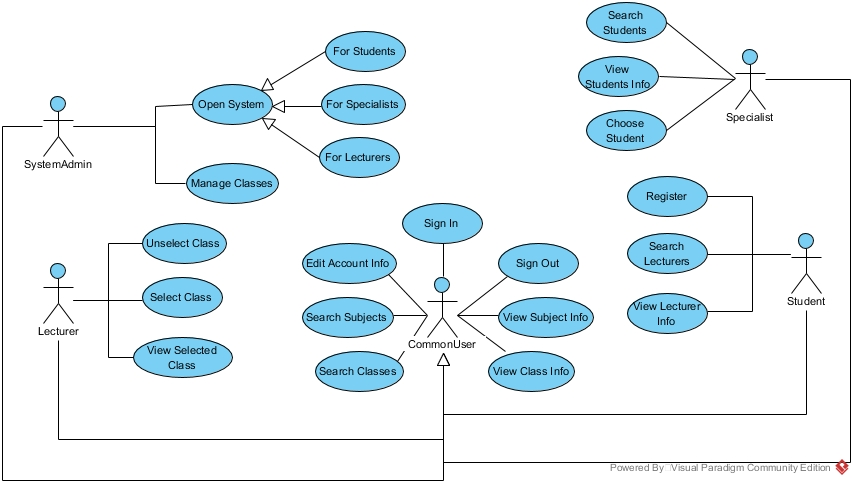
\includegraphics[scale=0.4]{../pictures/projectdiagrams/uc.jpg}
    \caption{Sơ đồ use case tổng quan}
  \end{figure}

  \paragraph{
    \textnormal{Do khả năng tận dụng diện tích có hạn nên một số use case được thể hiện trong các sơ đồ use case phân rã như dưới đây}
  }
  \clearpage

  \begin{figure}[!htb]
    \centering
    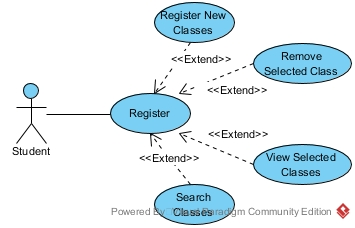
\includegraphics[scale=0.5]{../pictures/projectdiagrams/Register-uc-destructing.jpg}
    \caption{Sơ đồ phân rã cho use case đăng ký môn học}
  \end{figure}

  \begin{figure}[!htb]
    \centering
    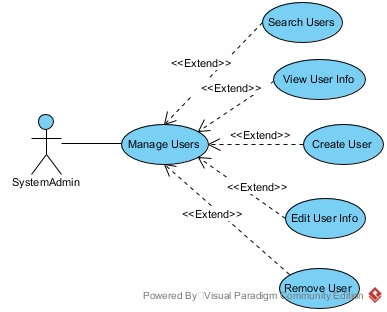
\includegraphics[scale=0.5]{../pictures/projectdiagrams/Manage-Users-uc-destructing.jpg}
    \caption{Sơ đồ phân rã cho use case quản lý người dùng}
  \end{figure}

  \begin{figure}[!htb]
    \centering
    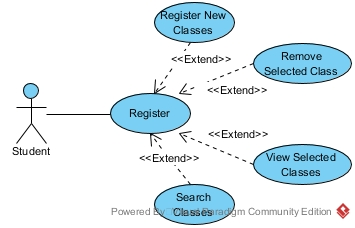
\includegraphics[scale=0.5]{../pictures/projectdiagrams/Manage-Subjects-uc-destructing.jpg}
    \caption{Sơ đồ phân rã cho use case quản lý môn học}
  \end{figure}

  \begin{figure}[!htb]
    \centering
    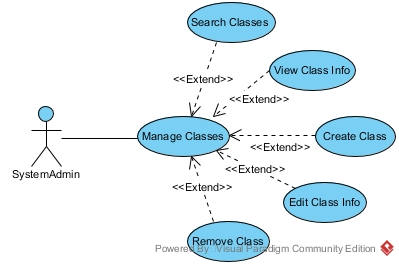
\includegraphics[scale=0.5]{../pictures/projectdiagrams/Manage-Classes-uc-destructing.jpg}
    \caption{Sơ đồ phân rã cho use case quản lý lớp học}
  \end{figure}

  \begin{figure}[!htb]
    \centering
    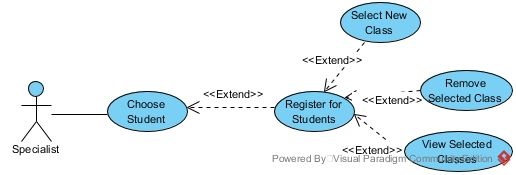
\includegraphics[scale=0.5]{../pictures/projectdiagrams/Choose-Student-uc-destructing.jpg}
    \caption{Sơ đồ phân rã cho use case chọn sinh viên}
  \end{figure}

  \clearpage % use this instead of \newpage or \pagebreak
  \subsection{Đặc tả use case dưới dạng bảng}

  \subsubsection*{Các use case chung}

  \begin{table}[ht]
    \centering
    \caption{\textbf{Đăng nhập}}
    \begin{tabularx}{\textwidth}{lXX}
      \toprule
      \textbf{Tên use case:} Đăng nhập & \multicolumn{2}{l}{\textbf{ID:} common01} \\
      \hline
      \multicolumn{3}{l}{\textbf{Tác nhân chính:} Tất cả} \\
      \hline
      \textbf{Mức độ quan trọng:} cao & \multicolumn{2}{l}{\textbf{Loại use case:} hệ thống} \\
      \hline
      \multicolumn{3}{l}{\textbf{Mô tả: }Xác thực người dùng dựa vào tên đăng nhập và mật khẩu} \\
      \hline
      \multicolumn{3}{p{0.95\textwidth}}{
        \textbf{Điều kiện khởi phát: }Người dùng truy cập vào hệ thống mà chưa được xác thực thành công.
      } \\
      \hline
      \multicolumn{3}{l}{
        \makecell[l]{
          \textbf{Quan hệ với các use case khác:}\\
          -- Để có thể thực hiện các use case khác, cần đăng nhập trước.
        }
      }\\
      \hline
      \multicolumn{3}{l}{\textbf{Luồng hoạt động chính:}} \\
      \hline
      TT $\qquad$ Thực hiện bởi & \multicolumn{2}{l}{Hành động} \\
      \hline
      $\quad 1\qquad\quad$ Người dùng & \multicolumn{2}{l}{Nhập thông tin đăng nhập} \\
      \hline
      $\quad 2\qquad\quad$ Người dùng & \multicolumn{2}{l}{Gửi yêu cầu đăng nhập} \\
      \hline
      $\quad 3\qquad\quad$ Hệ thống & \multicolumn{2}{l}{Kiểm tra thông tin đăng nhập} \\
      \hline
      $\quad 4\qquad\quad$ Hệ thống & \multicolumn{2}{l}{Điều hướng đến trang chính}\\
      \hline
      \multicolumn{3}{l}{\textbf{Luồng hoạt động con:}} \\
      \hline
      $\ 3.1\qquad\quad$ Hệ thống & \multicolumn{2}{l}{Thông báo thông tin đăng nhập sai} \\
      \bottomrule
    \end{tabularx}
  \end{table}

  \begin{table}[ht]
    \centering
    \caption{Đăng xuất}
    \begin{tabularx}{\textwidth}{lXX}
      \toprule
      \textbf{Tên use case:} Đăng xuất & \multicolumn{2}{l}{\textbf{ID:} common02} \\
      \hline
      \multicolumn{3}{l}{\textbf{Tác nhân chính:} Tất cả} \\
      \hline
      \textbf{Mức độ quan trọng:} trung bình & \multicolumn{2}{l}{\textbf{Loại use case:} hệ thống} \\
      \hline
      \multicolumn{3}{l}{\textbf{Mô tả: }Rời khỏi hệ thống} \\
      \hline
      \multicolumn{3}{p{0.95\textwidth}}{
        \textbf{Điều kiện khởi phát: }Người dùng yêu cầu đăng xuất
      } \\
      \hline
      \multicolumn{3}{l}{
        \makecell[l]{
          \textbf{Quan hệ với các use case khác:}\\
          -- Phụ thuộc vào use case đăng nhập.
        }
      }\\
      \hline
      \multicolumn{3}{l}{\textbf{Luồng hoạt động chính:}} \\
      \hline
      TT $\qquad$ Thực hiện bởi & \multicolumn{2}{l}{Hành động} \\
      \hline
      $\quad 1\qquad\quad$ Người dùng & \multicolumn{2}{l}{Chọn đăng xuất} \\
      \hline
      $\quad 2\qquad\quad$ Hệ thống & \multicolumn{2}{l}{Xóa session/cookie} \\
      \bottomrule
    \end{tabularx}
  \end{table}
  
  \begin{table}[ht]
    \centering
    \caption{Sửa thông tin tài khoản}
    \begin{tabularx}{\textwidth}{lXX}
      \toprule
      \multicolumn{2}{l}{\textbf{Tên use case: }Sửa thông tin tài khoản} & \textbf{ID: }common03 \\
      \hline
      \multicolumn{3}{l}{\textbf{Tác nhân chính: }Tất cả} \\
      \hline
      \textbf{Mức độ quan trọng: }trung bình & \multicolumn{2}{l}{\textbf{Loại use case: }hệ thống} \\
      \hline
      \multicolumn{3}{l}{\textbf{Mô tả: }Sửa các thông tin như \textit{thông tin cá nhân}, \textit{email}, \textit{mật khẩu}, \ldots} \\
      \hline
      \multicolumn{3}{l}{
        \textbf{Điều kiện khởi phát: }Người dùng truy cập trang chỉnh sửa thông tin tài khoản
      } \\
      \hline
      \multicolumn{3}{l}{
        \makecell[l]{
          \textbf{Quan hệ với các use case khác:} \\
          -- Phụ thuộc vào use case đăng nhập.
        }
      } \\
      \hline
      \multicolumn{3}{l}{\textbf{Luồng hoạt động chính:}} \\
      \hline
      TT $\qquad$ Thực hiện bởi & \multicolumn{2}{l}{Hành động} \\
      \hline
      $\quad 1\qquad\quad$ Người dùng & \multicolumn{2}{l}{Nhập lại những thông tin cần chỉnh sửa} \\
      \hline
      $\quad 2\qquad\quad$ Người dùng & \multicolumn{2}{l}{Gửi yêu cầu sửa} \\
      \hline
      $\quad 3\qquad\quad$ Hệ thống & \multicolumn{2}{l}{Kiểm tra tính hợp lý của thông tin mới} \\
      \hline
      $\quad 4\qquad\quad$ Hệ thống & \multicolumn{2}{l}{Cập nhật thông tin mới} \\
      \bottomrule
    \end{tabularx}
  \end{table}

  \newpage
  \subsubsection*{Dành cho quản trị hệ thống}
  
  \begin{table}[ht]
    \centering
    \caption{Đóng/mở hệ thống cho giảng viên}
    \begin{tabularx}{\textwidth}{lXX}
      \toprule
      \multicolumn{2}{l}{\textbf{Tên use case: }Đóng/mở hệ thống cho giảng viên} & \textbf{ID: }sa01 \\
      \hline
      \multicolumn{3}{l}{\textbf{Tác nhân chính: }quản trị hệ thống} \\
      \hline
      \textbf{Mức độ quan trọng: }cao & \multicolumn{2}{l}{\textbf{Loại use case: }hệ thống} \\
      \hline
      \multicolumn{3}{l}{\textbf{Mô tả: }Cho phép giảng viên chọn lớp} \\
      \hline
      \multicolumn{3}{l}{\textbf{Điều kiện khởi phát: }Quản trị viên chọn chức năng} \\
      \hline
      \multicolumn{3}{l}{
        \makecell[l]{
          \textbf{Quan hệ với các use case khác:}\\
          -- Phụ thuộc vào use case đăng nhập.
        }
      } \\
      \hline
      \multicolumn{3}{l}{\textbf{Luồng hoạt động chính:}} \\
      \hline
      TT $\qquad$ Thực hiện bởi & Hành động \\
      \hline
      $\quad 1\qquad\quad$ Quản trị hệ thống & \multicolumn{2}{l}{
        \makecell[l]{
          Chọn chức năng đóng hoặc mở hệ thống đối với\\ giảng viên}
      } \\
      \hline
      $\quad 2\qquad\quad$ Hệ thống & \multicolumn{2}{l}{Đóng hệ thống đối với các tác nhân khác} \\
      \hline
      \multicolumn{3}{l}{\textbf{Luồng hoạt động con:}} \\
      \hline
      $\ 1.1\qquad\quad$ Hệ thống & \multicolumn{2}{l}{Đóng hệ thống đối với giảng viên} \\
      \bottomrule
    \end{tabularx}
  \end{table}

  \begin{table}[ht]
    \centering
    \caption{Đóng/mở hệ thống cho chuyên viên}
    \begin{tabularx}{\textwidth}{lXX}
      \toprule
      \multicolumn{2}{l}{
        \textbf{Tên use case: }Đóng/mở hệ thống cho chuyên viên
      } & \textbf{ID: }sa02 \\
      \hline
      \multicolumn{3}{l}{\textbf{Tác nhân chính: }quản trị hệ thống} \\
      \hline
      \textbf{Mức độ quan trọng: }cao & \multicolumn{2}{l}{\textbf{Loại use case: }hệ thống} \\
      \hline
      \multicolumn{3}{l}{
        \makecell[l]{
          \textbf{Mô tả: }Cho phép chuyên viên thực hiện đăng ký lớp học/chỉnh sửa đăng ký giúp\\ sinh viên
        }
      }\\
      \hline
      \multicolumn{3}{l}{
        \makecell[l]{
          \textbf{Điều kiện khởi phát: }Quản trị viên chọn chức năng}
        } \\
      \hline
      \multicolumn{3}{l}{
        \makecell[l]{
          \textbf{Quan hệ với các use case khác:}\\
          -- Phụ thuộc vào use case đăng nhập
        }
      }\\
      \hline
      \multicolumn{3}{l}{\textbf{Luồng hoạt động chính:}} \\
      \hline
      TT $\qquad$ Thực hiện bởi & \multicolumn{2}{l}{Hành động} \\
      \hline
      $\quad 1\qquad\quad$ Quản trị hệ thống & \multicolumn{2}{l}{
        \makecell[l]{Chọn chức năng đóng hoặc mở hệ thống đối với\\ chuyên viên}} \\
      \hline
      $\quad 2\qquad\quad$ Hệ thống & \multicolumn{2}{l}{Đóng hệ thống đối với giảng viên} \\
      \hline
      $\quad 3\qquad\quad$ Hệ thống & \multicolumn{2}{l}{Mở hệ thống đối với chuyên viên} \\
      \hline
      \multicolumn{3}{l}{\textbf{Luồng hoạt động con:}} \\
      \hline
      $\ 1.1\qquad\quad$ Hệ thống & \multicolumn{2}{l}{Đóng hệ thống đối với chuyên viên} \\
      \bottomrule
    \end{tabularx}
  \end{table}

  \begin{table}[ht]
    \centering
    \caption{Đóng/mở hệ thống cho sinh viên}
    \begin{tabularx}{\textwidth}{lXX}
      \toprule
      \multicolumn{2}{l}{
        \textbf{Tên use case: }Đóng/mở hệ thống cho sinh viên
      } & \textbf{ID: }sa03 \\
      \hline
      \multicolumn{3}{l}{
        \textbf{Tác nhân chính: } quản trị hệ thống
      } \\
      \hline
      \textbf{Mức độ quan trọng: }cao & \multicolumn{2}{l}{\textbf{Loại use case: }hệ thống} \\
      \hline
      \multicolumn{3}{l}{
        \makecell[l]{
          \textbf{Mô tả: }Cho phép sinh viên đăng ký lớp học
        }
      } \\
      \hline
      \multicolumn{3}{l}{
        \textbf{Điều kiện khởi phát: }Quản trị viên chọn chức năng
      } \\
      \hline
      \multicolumn{3}{l}{
        \makecell[l]{
          \textbf{Quan hệ với các use case khác:}\\
          -- Phụ thuộc vào use case đăng nhập.
        }
      }\\
      \hline
      \multicolumn{3}{l}{\textbf{Luồng hoạt động chính:}}\\
      \hline
      TT $\quad\qquad$ Thực hiện bởi & Hành động \\
      \hline
      $\quad 1\qquad\quad$ Quản trị hệ thống & \multicolumn{2}{l}{
        \makecell[l]{
          Chọn chức năng đóng hoặc mở hệ thống đối với\\
          sinh viên
        }
      } \\
      \hline
      $\quad 2\qquad\quad$ Hệ thống & \multicolumn{2}{l}{Đóng hệ thống đối với giảng viên} \\
      \hline
      $\quad 3\qquad\quad$ Hệ thống & \multicolumn{2}{l}{Mở hệ thống đối với sinh viên} \\
      \hline
      \multicolumn{3}{l}{\textbf{Luồng hoạt động con:}} \\
      \hline
      $\ 1.1\qquad\quad$ Hệ thống & \multicolumn{2}{l}{Đóng hệ thống đối với sinh viên} \\
      \bottomrule
    \end{tabularx}
  \end{table}

  \newpage
  \subsubsection*{Dành cho sinh viên}

  \newpage
  \subsubsection*{Dành cho chuyên viên}

  \newpage
  \subsubsection*{Dành cho giảng viên}

  \subsection{Sơ đồ hoạt động}

\section{Phân tích tĩnh}

  \subsection{Xác định lớp}

  \subsection{Quan hệ giữa các lớp}

  \subsection{Lớp phân tích}

  \subsection{Xác định thuộc tính}

  \subsection{Xác định phương thức}

\section{Phân tích động}

  \subsection{Sơ đồ tuần tự}

\end{document}
